\titre{}
\theme{dérivées}
\auteur{Nathan Scheinmann}
\niveau{3M}
\source{fundamentum}
\type{serie}
\piments{2}
\pts{}
\annee{2425}

\contenu{
\tcblower
On construit une boîte rectangulaire en découpant quatre carrés aux coins d'une feuille de carton mesurant 32 cm sur 20 cm. Déterminer la hauteur $x$ de la boîte de volume maximal.
\begin{center}
\begin{tikzpicture}[scale=0.6]
    \tkzDefPoint(0,0){A} \tkzDefPoint(8,0){B}
    \tkzDefPoint(8,5){C} \tkzDefPoint(0,5){D}
    \tkzDrawPolygon(A,B,C,D);
    \tkzDrawSegment[dim={ $32$,0.5cm,}](D,C)
    \tkzDrawSegment[dim={ $20$,-0.5cm,}](D,A)
    \tkzDefPoint(1,1){A1} \tkzDefPoint(7,1){B1}
    \tkzDefPoint(7,4){C1} \tkzDefPoint(1,4){D1}
    \tkzDrawSegment[dashed](A1,B1)
    \tkzDrawSegment[dashed](B1,C1)
    \tkzDrawSegment[dashed](C1,D1)
    \tkzDrawSegment[dashed](D1,A1)

    \tkzDefPoint(0,1){L1} \tkzDefPoint(1,0){L2}
    \tkzDrawSegments(L1,A1 L2,A1);

    \tkzDefPoint(8,1){R1} \tkzDefPoint(7,0){R2}
    \tkzDrawSegments(R1,B1 R2,B1);

    \tkzDrawSegment[dim={ $x$,-0.5cm,}](R2,B)
    \tkzDrawSegment[dim={ $x$,-0.5cm,}](B,R1)

    \tkzDefPoint(0,4){L3} \tkzDefPoint(1,5){L4}
    \tkzDrawSegments(L3,D1 L4,D1);

    \tkzDefPoint(8,4){R3} \tkzDefPoint(7,5){R4}
    \tkzDrawSegments(R3,C1 R4,C1);
\end{tikzpicture}
\end{center}
}
\correction{
\tcblower
%% GENERATED BY AI %%
{\scriptsize \textit{Correction générée par IA}}

Après avoir découpé les carrés de côté $x$ aux coins, la boîte aura :
\begin{itemize}
\item Longueur : $32 - 2x$
\item Largeur : $20 - 2x$
\item Hauteur : $x$
\end{itemize}

Le volume est :
\[V(x) = x(32 - 2x)(20 - 2x) = x(640 - 64x - 40x + 4x^2) = x(640 - 104x + 4x^2)\]
\[= 4x^3 - 104x^2 + 640x\]

Pour maximiser le volume, dérivons :
\[V'(x) = 12x^2 - 208x + 640 = 4(3x^2 - 52x + 160)\]

Annulation :
\[3x^2 - 52x + 160 = 0\]

En utilisant la formule quadratique :
\[x = \frac{52 \pm \sqrt{52^2 - 4 \cdot 3 \cdot 160}}{2 \cdot 3} = \frac{52 \pm \sqrt{2704 - 1920}}{6} = \frac{52 \pm \sqrt{784}}{6} = \frac{52 \pm 28}{6}\]

Deux solutions : $x = \frac{80}{6} = \frac{40}{3} \approx 13{,}33$ ou $x = \frac{24}{6} = 4$.

Vérifions les contraintes : $x < 10$ (car $20 - 2x > 0$).

Donc $x = \frac{40}{3}$ est impossible, et la solution est $\boxed{x = 4 \text{ cm}}$.

Vérification : $V(4) = 4 \cdot 24 \cdot 12 = 1152$ cm$^3$.
}

